
\section{Equilibrium}
 As mentioned in the introduction, a board has reached quilibrium after $g$ generations if no  person has moved in the $g+1$-th generation.\\
In this parapgraph a portion of the first research question will be answered. Namely, will a board always reach an equilibrium in finite time? Based on intuition, this is expected to be true. An individual who moves, will move to a place where relatively more neighbours share his/her type, intuitively, this should imply that the average happiness of the population increases during each generation. In the basic model this is not always true however. Even though equilibrium is nearly alays reached in finite time, there exists cases in which allow a periodic solution. One example of any such scenario is given below:\\

\begin{figure}[H]
    \centering
    \begin{subfigure}{0.3\textwidth}
        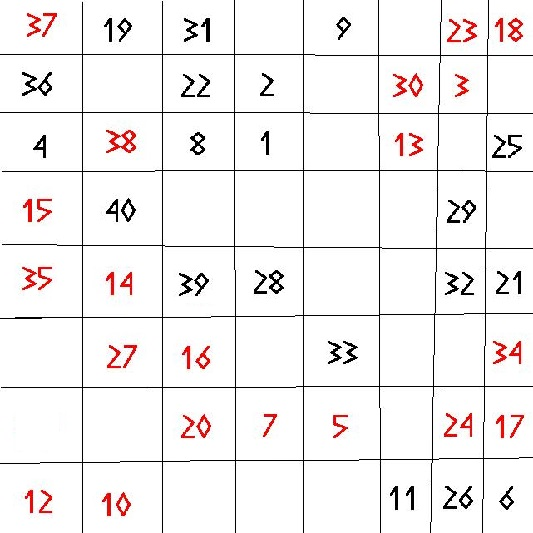
\includegraphics[width=\textwidth]{Tegenvoorbeeld/segregation_tegenvb.jpg}
        \caption{The start situation. Individual $37$ will move.}
        \label{fig:movement1}
    \end{subfigure}\hspace{1cm}
    ~ %add desired spacing between images, e. g. ~, \quad, \qquad, \hfill etc. 
      %(or a blank line to force the subfigure onto a new line)
    \begin{subfigure}{0.3\textwidth}
        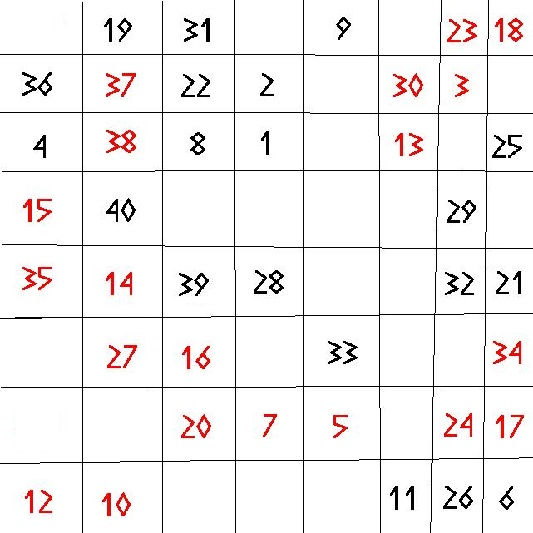
\includegraphics[width=\textwidth]{Tegenvoorbeeld/segregation_tegenvb_1.jpg}
        \caption{Individual $37$ is moved to the nearest location that better meets his/her desires. }
        \label{fig:movement2}
    \end{subfigure}
    ~ %add desired spacing between images, e. g. ~, \quad, \qquad, \hfill etc. 
    %(or a blank line to force the subfigure onto a new line)
    \begin{subfigure}{0.3\textwidth}
        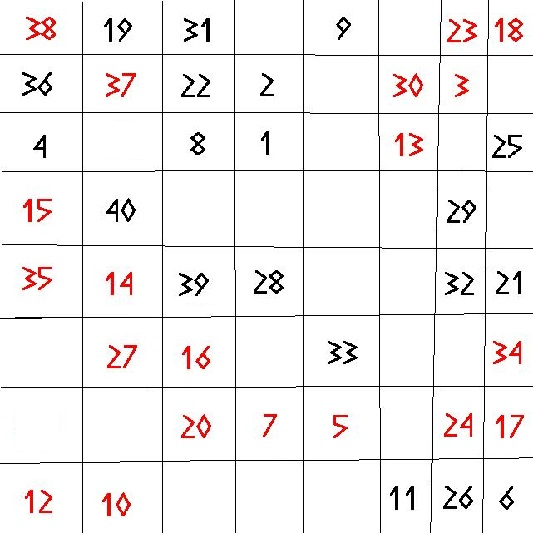
\includegraphics[width=\textwidth]{Tegenvoorbeeld/segregation_tegenvb_2.jpg}
        \caption{Accordingly, $38$ will move next and is moved to the nearest location that better meets his/her desires.}
        \label{fig:movement3}
    \end{subfigure}\hspace{1cm}
    \begin{subfigure}{0.3\textwidth}
        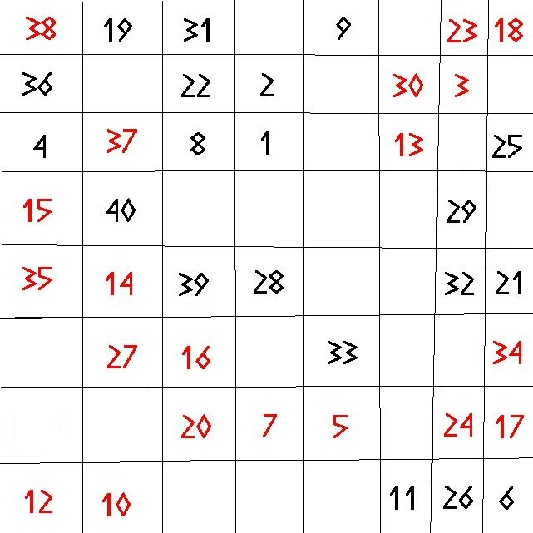
\includegraphics[width=\textwidth]{Tegenvoorbeeld/segregation_tegenvb_3.jpg}
        \caption{A generation has passed, $37$ is next to move and will do so accordingly. The roles of  $37$ and $38$ have interchanged, which leads to a periodic solution. }
        \label{fig:movement4}
    \end{subfigure}
    \caption{A possible configuration of the standard board in which the equilibrium will never be reached. The numbers indicate the turn order of an individuals. The two different colour indicates the two types. The equilibrium is not reached due to the periodic movements of individuals $37$ and $38$. The movements of inviduals $37$ and $38$ are tracked and shown in subfigure a to d in a chronological order.}\label{fig:equilibrium counterexample}
\end{figure}



In figure \ref{fig:equilibrium counterexample}, a possible configuration in which  equilibrium will not be reached is shown. The numbers represent the turn order ($1$ is selected first followed by $2$, etc.). Red and black indicate  the two different types. It is easily observed that that individuals $1$ to $36$ satisfy the happiness condition. $37$ however does not. During $37$'s turn, we note that his/her happiness equals $0$. The closest empty location has a happiness of $\frac{1}{7} > 0$. And thus $37$ will move to the given location, which is indicated in figure \ref{fig:movement2}.
\\Next in line to move is $38$. $38$ has a happiness of $\frac{2}{7}$, which is less than the required $\frac{1}{3}$ and will thus have to move. The closest spot with greater happiness is the nearby corner spot with happiness $\frac{1}{3}$. So $38$ move to that location, which is shown in figure \ref{fig:movement3}.\\
The indviduals \(1\) to \(36\) will remain pleased and will thus remain in place. Thus  $37$ is the first candidate to be moved. $37$ has a happiness $\frac{1}{7} < \frac{1}{3}$. The closest empty spot has happiness $\frac{1}{6} > \frac{1}{7}$, thus $37$ will move to this location. Since this location was te former spot of \(38\), we conclude that  $37$ and $38$ have swapped positions, as is shown in figure \ref{fig:movement4}.\\
Since $37$ and $38$ are of the same type, these $3$ moves will continue periodically and thus we find a periodic solution.\\
\textbf{Now what went wrong?} After the first move, both $37$ and $38$ will gain happiness, but as \(37\) moves away, $38$ will loses all of his/her happiness. 
An endless loop is formed.\\
Note that, the same scenario can be constructed for larger boards. Since we can implement this exact board in a larger board and fill out the remaining locations to satisfy an equilibrium.
